\documentclass[__main__.tex]{subfiles}

\begin{document}

\qtitle{С}{04}
Покажите, что напряженность электростатического поля точечного диполя имеет вид $\vec{E} = \frac{1}{4\pi\varepsilon_0}\left( 3\frac{\left<\vec{p}_e, \vec{r}\right>}{r^5}\vec{r} - \frac{\vec{p}_e}{r^3}\right)$, где $\vec{r}$ радиус-вектор, проведённый из диполя в точку наблюдения, $\vec{p}_{e}$ -- электрический дипольный момент.\\ 
\begin{definition}
Электрический диполь–система двух разноименных по знаку и одинаковых  по  величине  точечных  зарядов,  находящихся  на небольшом расстоянии один от другого.\\
\end{definition}
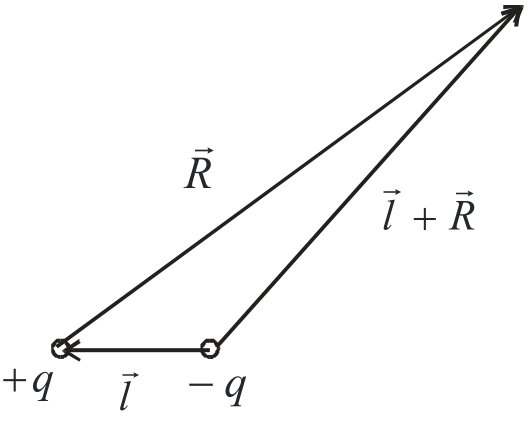
\includegraphics[scale=0.5]{C4_1}\\
Начнем с нахождения потенциала диполя:\\
\begin{gather}
\phi(\vec{r}) = \frac{1}{4\pi \epsilon_0}\left(\frac{q}{r}-\frac{r}{|\vec{r}+\vec{l}|}\right),
\end{gather}
где $q>0$.
\begin{gather}
\frac{1}{|\vec{r}+\vec{l}|} = \frac{1}{\sqrt{(\vec{r}+\vec{l})^2}} = \frac{1}{\sqrt{r^2+2\vec{r}\vec{l}+l^2}} = \frac{1}{r\sqrt{1+2\frac{\vec{r}\vec{l}}{r^2}+\frac{l^2}{r^2}}}\approx \frac{1}{r}-\frac{\vec{r}\vec{l}}{r^3} \\ \Longrightarrow \phi(\vec{r}) = \frac{1}{4 \pi \epsilon_0}\frac{\vec{p}_{e}\vec{r}}{r^3},
\end{gather}
где $\vec{p}_{e} = q\vec{l}$ - электрический дипольный момент.\\
Тогда напряженность электростатического поля точечного диполя:\\
\begin{gather}
\vec{E} = -\nabla \phi, E_x = -\frac{\partial}{\partial x}\phi = -\frac{\partial}{\partial x}k \frac{\vec{p}_{e}\vec{r}}{r^3} = -\frac{\partial}{\partial x}k\frac{p_{ex}x+p_{ey}y+p_{ez}z}{\sqrt{(x^2+y^2+z^2)^3}} =\\ -k(\vec{p}_{e}\vec{r})\left(-\frac{3}{2}\right)\frac{2x}{r^5}-k\frac{p_{ex}}{r^3} = k\left(\frac{3(\vec{p}_{e}\vec{r})x}{r^5}-\frac{p_{ex}}{r^3}\right)\\
\vec{E} = \frac{1}{4 \pi \epsilon_0}\left( 3\frac{\left<\vec{p}_e, \vec{r}\right>}{r^5}\vec{r} - \frac{\vec{p}_e}{r^3}\right)
\end{gather}
На протяжении вывода мы использовали коэффициент $k = \frac{1}{4 \pi \epsilon_0}$, прям как тот, что в законе Кулона.
%%

\end{document}